\documentclass[12pt]{article}
\usepackage[letterpaper, left=0.6in, right=0.6in, top=0.95in, bottom=0.95in,
  headheight=15pt, headsep=0.25in, footskip=0.45in]{geometry}
\usepackage[T1]{fontenc}
\usepackage[default]{sourcesanspro}
\usepackage{inconsolata}
\usepackage{textcomp}
\usepackage{microtype}
\usepackage{tikz}
\usetikzlibrary{arrows.meta}
\usepackage{fancyhdr}
\pagestyle{fancy}
\fancyhf{}
\fancyhead[L]{Week 4 / Stars and wheels / Grades 4--5}
\fancyfoot[L]{Bellingham Math Circle / Week 4 / F04-U-v4}
\fancyfoot[R]{\thepage}
\renewcommand{\headrulewidth}{0pt}
\setlength{\parindent}{0pt}
\setlength{\parskip}{0pt}
\newcommand{\prob}[1]{\textbf{Problem #1:}}
\newcommand{\bx}{\hspace{0.07in}\begingroup\setlength{\fboxsep}{0pt}\setlength{\fboxrule}{0.8pt}\raisebox{-0.11in}{\framebox[0.42in]{\rule{0pt}{0.34in}}}\endgroup}
\newcommand{\blank}{\rule[-3pt]{0.85in}{0.6pt}}
\pagenumbering{arabic}
\begin{document}
\par\vspace{0in}\noindent To draw hop 3 on a ring of dots, start at any dot and draw a straight line to the dot 3 places clockwise. Keep hopping 3 until you are back where you started. If some dots still have no line, start again at one of them, and stop when every dot has a line. The lines you draw from one start make one piece.\par
\par\vspace{0.16in}\noindent \prob{1} Draw hops 1 to 6 on these rings of 12 dots. Write how many pieces each drawing has.\par
\par\vspace{0.3in}\noindent\makebox[\textwidth][s]{\hfill 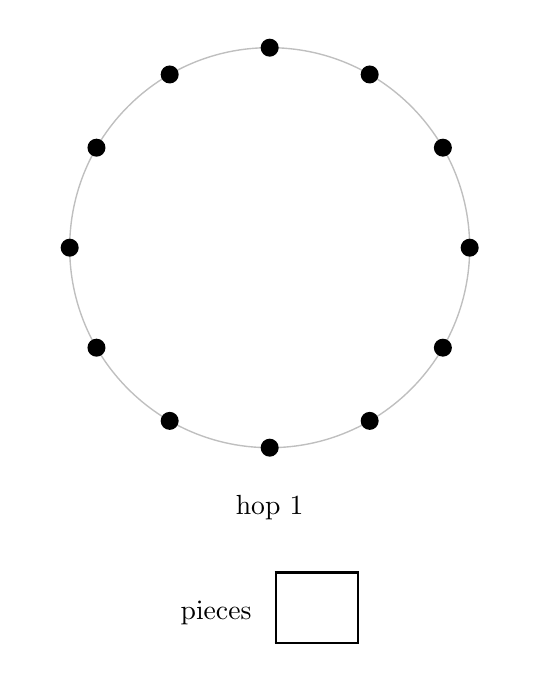
\begin{tikzpicture}[x=1in,y=1in]
\useasboundingbox (-1.21,-2.1) rectangle (1.21,1.1);
\draw[black!25, line width=0.5pt] (0,0) circle (1);
\fill[black] (0,1) circle (0.045);
\fill[black] (0.5,0.866) circle (0.045);
\fill[black] (0.866,0.5) circle (0.045);
\fill[black] (1,0) circle (0.045);
\fill[black] (0.866,-0.5) circle (0.045);
\fill[black] (0.5,-0.866) circle (0.045);
\fill[black] (0,-1) circle (0.045);
\fill[black] (-0.5,-0.866) circle (0.045);
\fill[black] (-0.866,-0.5) circle (0.045);
\fill[black] (-1,0) circle (0.045);
\fill[black] (-0.866,0.5) circle (0.045);
\fill[black] (-0.5,0.866) circle (0.045);
\node[font=\normalsize] at (0,-1.3) {hop 1};
\node[font=\normalsize] at (0,-1.8) {pieces~\bx};
\end{tikzpicture}\hfill 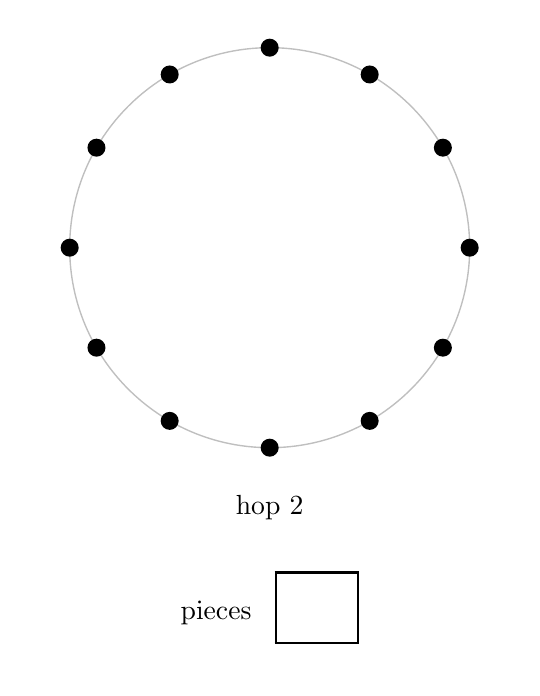
\begin{tikzpicture}[x=1in,y=1in]
\useasboundingbox (-1.21,-2.1) rectangle (1.21,1.1);
\draw[black!25, line width=0.5pt] (0,0) circle (1);
\fill[black] (0,1) circle (0.045);
\fill[black] (0.5,0.866) circle (0.045);
\fill[black] (0.866,0.5) circle (0.045);
\fill[black] (1,0) circle (0.045);
\fill[black] (0.866,-0.5) circle (0.045);
\fill[black] (0.5,-0.866) circle (0.045);
\fill[black] (0,-1) circle (0.045);
\fill[black] (-0.5,-0.866) circle (0.045);
\fill[black] (-0.866,-0.5) circle (0.045);
\fill[black] (-1,0) circle (0.045);
\fill[black] (-0.866,0.5) circle (0.045);
\fill[black] (-0.5,0.866) circle (0.045);
\node[font=\normalsize] at (0,-1.3) {hop 2};
\node[font=\normalsize] at (0,-1.8) {pieces~\bx};
\end{tikzpicture}\hfill 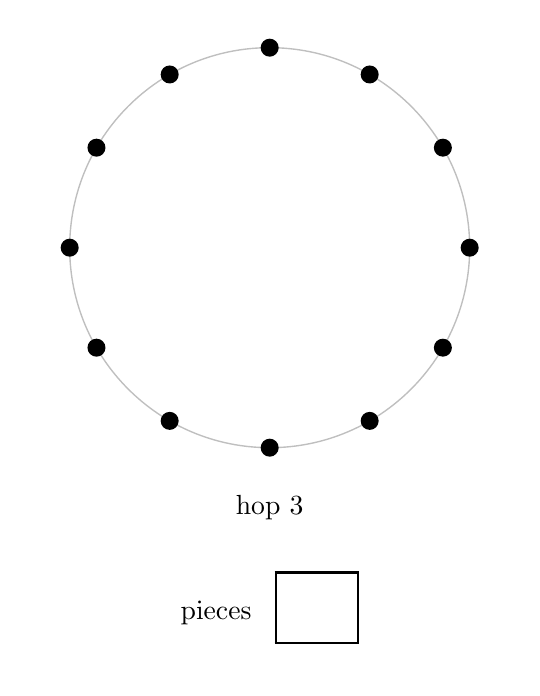
\begin{tikzpicture}[x=1in,y=1in]
\useasboundingbox (-1.21,-2.1) rectangle (1.21,1.1);
\draw[black!25, line width=0.5pt] (0,0) circle (1);
\fill[black] (0,1) circle (0.045);
\fill[black] (0.5,0.866) circle (0.045);
\fill[black] (0.866,0.5) circle (0.045);
\fill[black] (1,0) circle (0.045);
\fill[black] (0.866,-0.5) circle (0.045);
\fill[black] (0.5,-0.866) circle (0.045);
\fill[black] (0,-1) circle (0.045);
\fill[black] (-0.5,-0.866) circle (0.045);
\fill[black] (-0.866,-0.5) circle (0.045);
\fill[black] (-1,0) circle (0.045);
\fill[black] (-0.866,0.5) circle (0.045);
\fill[black] (-0.5,0.866) circle (0.045);
\node[font=\normalsize] at (0,-1.3) {hop 3};
\node[font=\normalsize] at (0,-1.8) {pieces~\bx};
\end{tikzpicture}\hfill}\par
\par\vspace{0.4in}\noindent\makebox[\textwidth][s]{\hfill 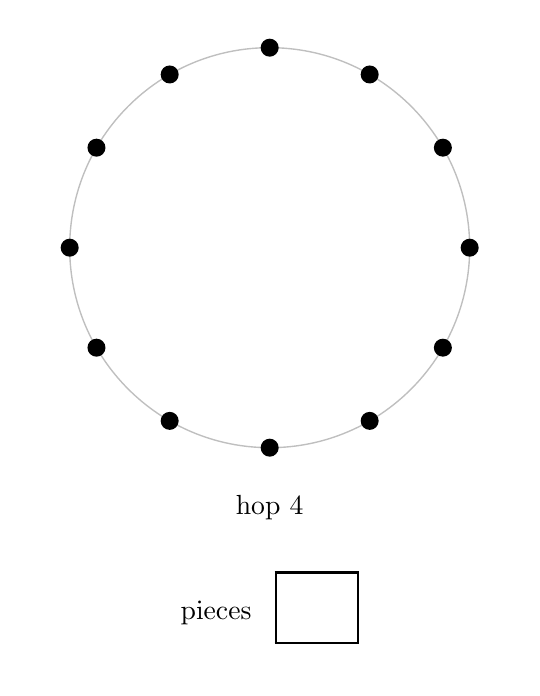
\begin{tikzpicture}[x=1in,y=1in]
\useasboundingbox (-1.21,-2.1) rectangle (1.21,1.1);
\draw[black!25, line width=0.5pt] (0,0) circle (1);
\fill[black] (0,1) circle (0.045);
\fill[black] (0.5,0.866) circle (0.045);
\fill[black] (0.866,0.5) circle (0.045);
\fill[black] (1,0) circle (0.045);
\fill[black] (0.866,-0.5) circle (0.045);
\fill[black] (0.5,-0.866) circle (0.045);
\fill[black] (0,-1) circle (0.045);
\fill[black] (-0.5,-0.866) circle (0.045);
\fill[black] (-0.866,-0.5) circle (0.045);
\fill[black] (-1,0) circle (0.045);
\fill[black] (-0.866,0.5) circle (0.045);
\fill[black] (-0.5,0.866) circle (0.045);
\node[font=\normalsize] at (0,-1.3) {hop 4};
\node[font=\normalsize] at (0,-1.8) {pieces~\bx};
\end{tikzpicture}\hfill 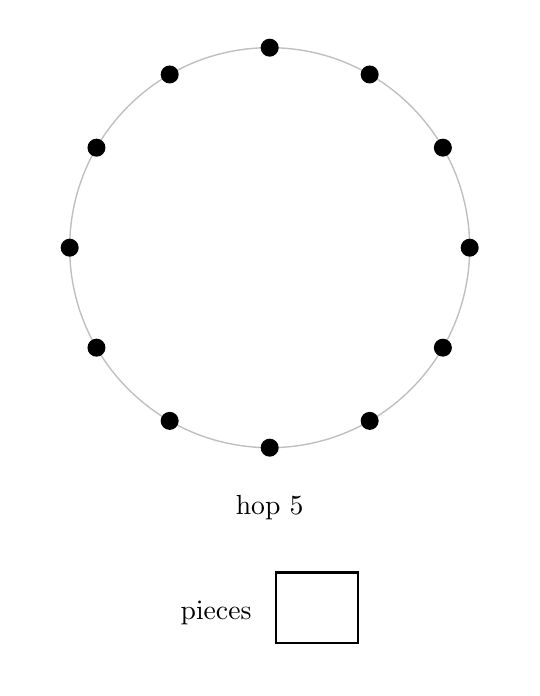
\begin{tikzpicture}[x=1in,y=1in]
\useasboundingbox (-1.21,-2.1) rectangle (1.21,1.1);
\draw[black!25, line width=0.5pt] (0,0) circle (1);
\fill[black] (0,1) circle (0.045);
\fill[black] (0.5,0.866) circle (0.045);
\fill[black] (0.866,0.5) circle (0.045);
\fill[black] (1,0) circle (0.045);
\fill[black] (0.866,-0.5) circle (0.045);
\fill[black] (0.5,-0.866) circle (0.045);
\fill[black] (0,-1) circle (0.045);
\fill[black] (-0.5,-0.866) circle (0.045);
\fill[black] (-0.866,-0.5) circle (0.045);
\fill[black] (-1,0) circle (0.045);
\fill[black] (-0.866,0.5) circle (0.045);
\fill[black] (-0.5,0.866) circle (0.045);
\node[font=\normalsize] at (0,-1.3) {hop 5};
\node[font=\normalsize] at (0,-1.8) {pieces~\bx};
\end{tikzpicture}\hfill 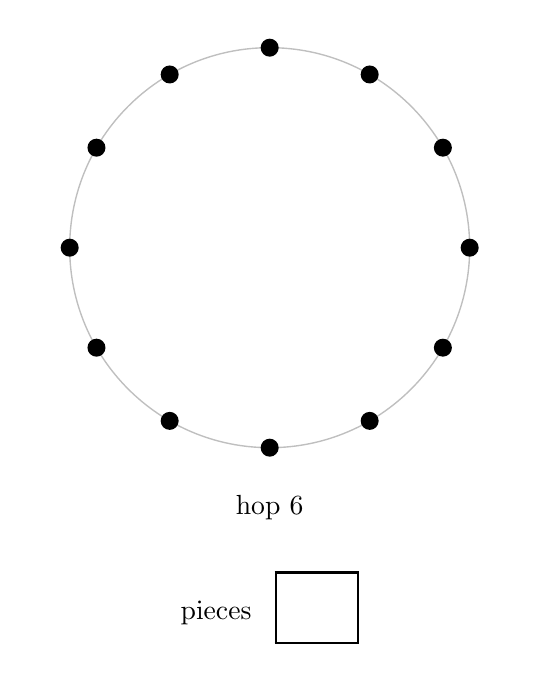
\begin{tikzpicture}[x=1in,y=1in]
\useasboundingbox (-1.21,-2.1) rectangle (1.21,1.1);
\draw[black!25, line width=0.5pt] (0,0) circle (1);
\fill[black] (0,1) circle (0.045);
\fill[black] (0.5,0.866) circle (0.045);
\fill[black] (0.866,0.5) circle (0.045);
\fill[black] (1,0) circle (0.045);
\fill[black] (0.866,-0.5) circle (0.045);
\fill[black] (0.5,-0.866) circle (0.045);
\fill[black] (0,-1) circle (0.045);
\fill[black] (-0.5,-0.866) circle (0.045);
\fill[black] (-0.866,-0.5) circle (0.045);
\fill[black] (-1,0) circle (0.045);
\fill[black] (-0.866,0.5) circle (0.045);
\fill[black] (-0.5,0.866) circle (0.045);
\node[font=\normalsize] at (0,-1.3) {hop 6};
\node[font=\normalsize] at (0,-1.8) {pieces~\bx};
\end{tikzpicture}\hfill}\par
\vfill

\newpage
\par\vspace{0in}\noindent \prob{2} Draw each of these, and write how many pieces it has.\par
\par\vspace{0.3in}\noindent\makebox[\textwidth][s]{\hfill 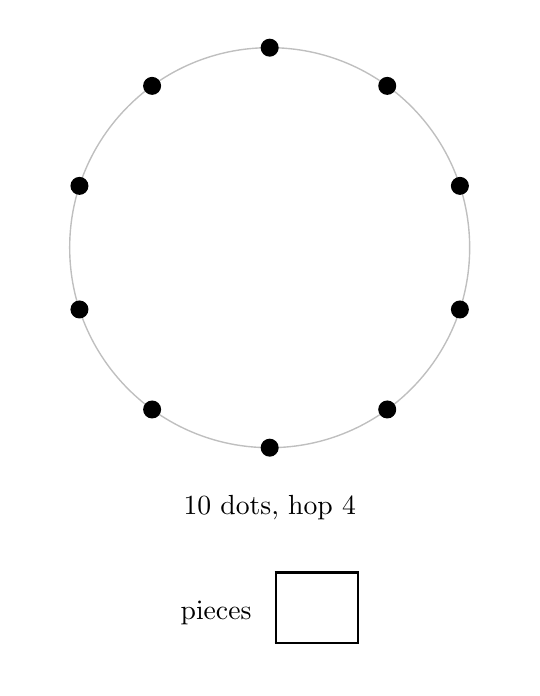
\begin{tikzpicture}[x=1in,y=1in]
\useasboundingbox (-1.21,-2.1) rectangle (1.21,1.1);
\draw[black!25, line width=0.5pt] (0,0) circle (1);
\fill[black] (0,1) circle (0.045);
\fill[black] (0.5878,0.809) circle (0.045);
\fill[black] (0.9511,0.309) circle (0.045);
\fill[black] (0.9511,-0.309) circle (0.045);
\fill[black] (0.5878,-0.809) circle (0.045);
\fill[black] (0,-1) circle (0.045);
\fill[black] (-0.5878,-0.809) circle (0.045);
\fill[black] (-0.9511,-0.309) circle (0.045);
\fill[black] (-0.9511,0.309) circle (0.045);
\fill[black] (-0.5878,0.809) circle (0.045);
\node[font=\normalsize] at (0,-1.3) {10 dots, hop 4};
\node[font=\normalsize] at (0,-1.8) {pieces~\bx};
\end{tikzpicture}\hfill \begin{tikzpicture}[x=1in,y=1in]
\useasboundingbox (-1.21,-2.1) rectangle (1.21,1.1);
\draw[black!25, line width=0.5pt] (0,0) circle (1);
\fill[black] (0,1) circle (0.045);
\fill[black] (0.6428,0.766) circle (0.045);
\fill[black] (0.9848,0.1736) circle (0.045);
\fill[black] (0.866,-0.5) circle (0.045);
\fill[black] (0.342,-0.9397) circle (0.045);
\fill[black] (-0.342,-0.9397) circle (0.045);
\fill[black] (-0.866,-0.5) circle (0.045);
\fill[black] (-0.9848,0.1736) circle (0.045);
\fill[black] (-0.6428,0.766) circle (0.045);
\node[font=\normalsize] at (0,-1.3) {9 dots, hop 6};
\node[font=\normalsize] at (0,-1.8) {pieces~\bx};
\end{tikzpicture}\hfill 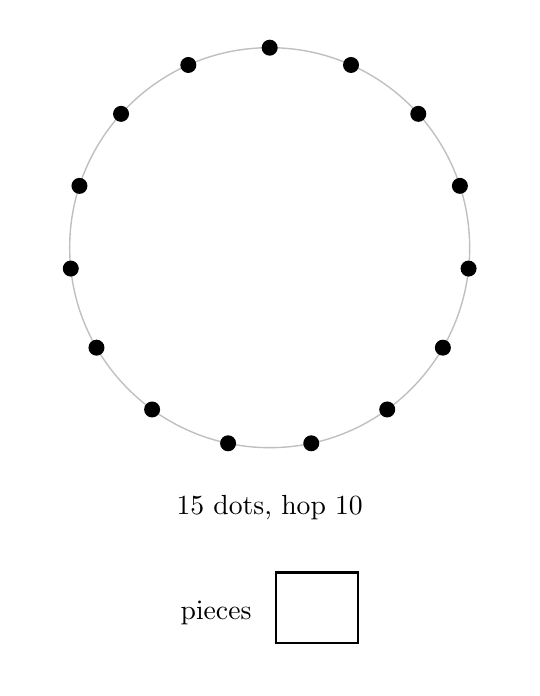
\begin{tikzpicture}[x=1in,y=1in]
\useasboundingbox (-1.21,-2.1) rectangle (1.21,1.1);
\draw[black!25, line width=0.5pt] (0,0) circle (1);
\fill[black] (0,1) circle (0.04);
\fill[black] (0.4067,0.9135) circle (0.04);
\fill[black] (0.7431,0.6691) circle (0.04);
\fill[black] (0.9511,0.309) circle (0.04);
\fill[black] (0.9945,-0.1045) circle (0.04);
\fill[black] (0.866,-0.5) circle (0.04);
\fill[black] (0.5878,-0.809) circle (0.04);
\fill[black] (0.2079,-0.9781) circle (0.04);
\fill[black] (-0.2079,-0.9781) circle (0.04);
\fill[black] (-0.5878,-0.809) circle (0.04);
\fill[black] (-0.866,-0.5) circle (0.04);
\fill[black] (-0.9945,-0.1045) circle (0.04);
\fill[black] (-0.9511,0.309) circle (0.04);
\fill[black] (-0.7431,0.6691) circle (0.04);
\fill[black] (-0.4067,0.9135) circle (0.04);
\node[font=\normalsize] at (0,-1.3) {15 dots, hop 10};
\node[font=\normalsize] at (0,-1.8) {pieces~\bx};
\end{tikzpicture}\hfill}\par
\par\vspace{0.45in}\noindent\makebox[\textwidth][s]{\hfill 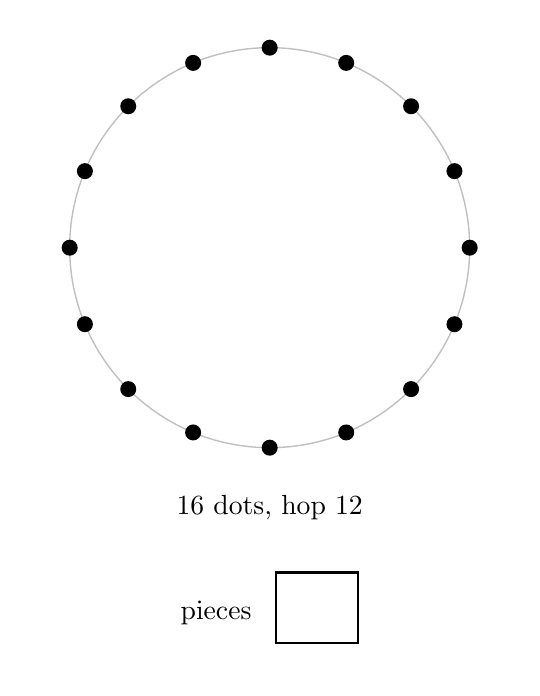
\begin{tikzpicture}[x=1in,y=1in]
\useasboundingbox (-1.21,-2.1) rectangle (1.21,1.1);
\draw[black!25, line width=0.5pt] (0,0) circle (1);
\fill[black] (0,1) circle (0.04);
\fill[black] (0.3827,0.9239) circle (0.04);
\fill[black] (0.7071,0.7071) circle (0.04);
\fill[black] (0.9239,0.3827) circle (0.04);
\fill[black] (1,0) circle (0.04);
\fill[black] (0.9239,-0.3827) circle (0.04);
\fill[black] (0.7071,-0.7071) circle (0.04);
\fill[black] (0.3827,-0.9239) circle (0.04);
\fill[black] (0,-1) circle (0.04);
\fill[black] (-0.3827,-0.9239) circle (0.04);
\fill[black] (-0.7071,-0.7071) circle (0.04);
\fill[black] (-0.9239,-0.3827) circle (0.04);
\fill[black] (-1,0) circle (0.04);
\fill[black] (-0.9239,0.3827) circle (0.04);
\fill[black] (-0.7071,0.7071) circle (0.04);
\fill[black] (-0.3827,0.9239) circle (0.04);
\node[font=\normalsize] at (0,-1.3) {16 dots, hop 12};
\node[font=\normalsize] at (0,-1.8) {pieces~\bx};
\end{tikzpicture}\hfill 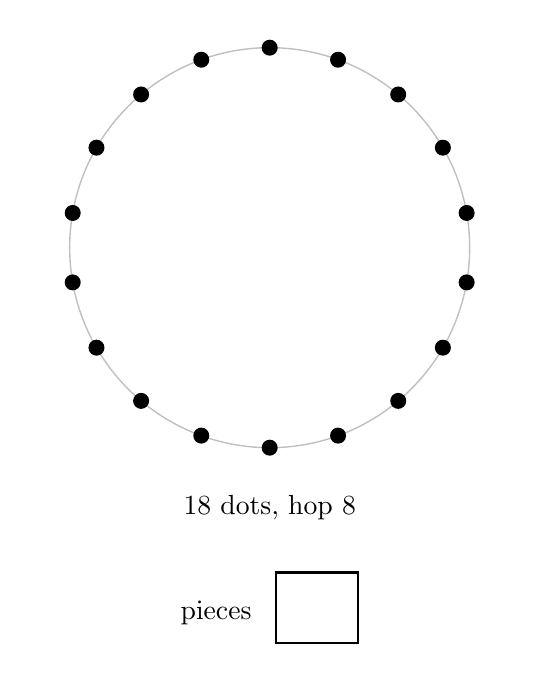
\begin{tikzpicture}[x=1in,y=1in]
\useasboundingbox (-1.21,-2.1) rectangle (1.21,1.1);
\draw[black!25, line width=0.5pt] (0,0) circle (1);
\fill[black] (0,1) circle (0.04);
\fill[black] (0.342,0.9397) circle (0.04);
\fill[black] (0.6428,0.766) circle (0.04);
\fill[black] (0.866,0.5) circle (0.04);
\fill[black] (0.9848,0.1736) circle (0.04);
\fill[black] (0.9848,-0.1736) circle (0.04);
\fill[black] (0.866,-0.5) circle (0.04);
\fill[black] (0.6428,-0.766) circle (0.04);
\fill[black] (0.342,-0.9397) circle (0.04);
\fill[black] (0,-1) circle (0.04);
\fill[black] (-0.342,-0.9397) circle (0.04);
\fill[black] (-0.6428,-0.766) circle (0.04);
\fill[black] (-0.866,-0.5) circle (0.04);
\fill[black] (-0.9848,-0.1736) circle (0.04);
\fill[black] (-0.9848,0.1736) circle (0.04);
\fill[black] (-0.866,0.5) circle (0.04);
\fill[black] (-0.6428,0.766) circle (0.04);
\fill[black] (-0.342,0.9397) circle (0.04);
\node[font=\normalsize] at (0,-1.3) {18 dots, hop 8};
\node[font=\normalsize] at (0,-1.8) {pieces~\bx};
\end{tikzpicture}\hfill 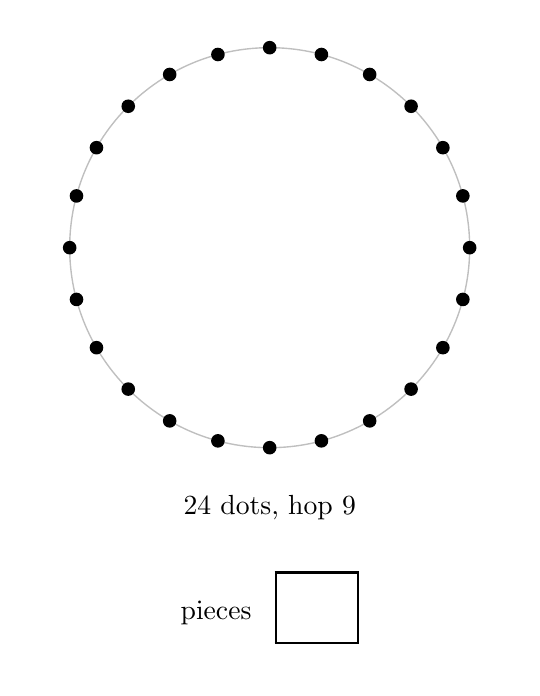
\begin{tikzpicture}[x=1in,y=1in]
\useasboundingbox (-1.21,-2.1) rectangle (1.21,1.1);
\draw[black!25, line width=0.5pt] (0,0) circle (1);
\fill[black] (0,1) circle (0.034);
\fill[black] (0.2588,0.9659) circle (0.034);
\fill[black] (0.5,0.866) circle (0.034);
\fill[black] (0.7071,0.7071) circle (0.034);
\fill[black] (0.866,0.5) circle (0.034);
\fill[black] (0.9659,0.2588) circle (0.034);
\fill[black] (1,0) circle (0.034);
\fill[black] (0.9659,-0.2588) circle (0.034);
\fill[black] (0.866,-0.5) circle (0.034);
\fill[black] (0.7071,-0.7071) circle (0.034);
\fill[black] (0.5,-0.866) circle (0.034);
\fill[black] (0.2588,-0.9659) circle (0.034);
\fill[black] (0,-1) circle (0.034);
\fill[black] (-0.2588,-0.9659) circle (0.034);
\fill[black] (-0.5,-0.866) circle (0.034);
\fill[black] (-0.7071,-0.7071) circle (0.034);
\fill[black] (-0.866,-0.5) circle (0.034);
\fill[black] (-0.9659,-0.2588) circle (0.034);
\fill[black] (-1,0) circle (0.034);
\fill[black] (-0.9659,0.2588) circle (0.034);
\fill[black] (-0.866,0.5) circle (0.034);
\fill[black] (-0.7071,0.7071) circle (0.034);
\fill[black] (-0.5,0.866) circle (0.034);
\fill[black] (-0.2588,0.9659) circle (0.034);
\node[font=\normalsize] at (0,-1.3) {24 dots, hop 9};
\node[font=\normalsize] at (0,-1.8) {pieces~\bx};
\end{tikzpicture}\hfill}\par
\vfill

\newpage
\par\vspace{0in}\noindent \prob{3} Find how many pieces each of these drawings has, without drawing it. Then draw the first two on the rings to check.\par
\par\vspace{0.3in}\noindent\makebox[\textwidth][c]{\begin{tikzpicture}[x=1in,y=1in]
\useasboundingbox (0,-6.6) rectangle (7.3,0.05);
\node[font=\normalsize, anchor=west] at (0,-0.3) {20 dots, hop 8};
\node[font=\normalsize, anchor=west] at (1.75,-0.3) {pieces};
\draw[black, line width=0.7pt] (2.4,-0.4) -- (3.2,-0.4);
\node[font=\normalsize, anchor=west] at (0,-0.9) {24 dots, hop 10};
\node[font=\normalsize, anchor=west] at (1.75,-0.9) {pieces};
\draw[black, line width=0.7pt] (2.4,-1) -- (3.2,-1);
\node[font=\normalsize, anchor=west] at (0,-1.5) {30 dots, hop 12};
\node[font=\normalsize, anchor=west] at (1.75,-1.5) {pieces};
\draw[black, line width=0.7pt] (2.4,-1.6) -- (3.2,-1.6);
\node[font=\normalsize, anchor=west] at (0,-2.1) {36 dots, hop 27};
\node[font=\normalsize, anchor=west] at (1.75,-2.1) {pieces};
\draw[black, line width=0.7pt] (2.4,-2.2) -- (3.2,-2.2);
\node[font=\normalsize, anchor=west] at (0,-2.7) {17 dots, hop 5};
\node[font=\normalsize, anchor=west] at (1.75,-2.7) {pieces};
\draw[black, line width=0.7pt] (2.4,-2.8) -- (3.2,-2.8);
\node[font=\normalsize, anchor=west] at (0,-3.3) {100 dots, hop 35};
\node[font=\normalsize, anchor=west] at (1.75,-3.3) {pieces};
\draw[black, line width=0.7pt] (2.4,-3.4) -- (3.2,-3.4);
\node[font=\normalsize, anchor=west] at (0,-3.9) {60 dots, hop 45};
\node[font=\normalsize, anchor=west] at (1.75,-3.9) {pieces};
\draw[black, line width=0.7pt] (2.4,-4) -- (3.2,-4);
\draw[black!25, line width=0.5pt] (5.45,-1.5) circle (1.38);
\fill[black] (5.45,-0.12) circle (0.038);
\fill[black] (5.8764,-0.1875) circle (0.038);
\fill[black] (6.2611,-0.3836) circle (0.038);
\fill[black] (6.5664,-0.6889) circle (0.038);
\fill[black] (6.7625,-1.0736) circle (0.038);
\fill[black] (6.83,-1.5) circle (0.038);
\fill[black] (6.7625,-1.9264) circle (0.038);
\fill[black] (6.5664,-2.3111) circle (0.038);
\fill[black] (6.2611,-2.6164) circle (0.038);
\fill[black] (5.8764,-2.8125) circle (0.038);
\fill[black] (5.45,-2.88) circle (0.038);
\fill[black] (5.0236,-2.8125) circle (0.038);
\fill[black] (4.6389,-2.6164) circle (0.038);
\fill[black] (4.3336,-2.3111) circle (0.038);
\fill[black] (4.1375,-1.9264) circle (0.038);
\fill[black] (4.07,-1.5) circle (0.038);
\fill[black] (4.1375,-1.0736) circle (0.038);
\fill[black] (4.3336,-0.6889) circle (0.038);
\fill[black] (4.6389,-0.3836) circle (0.038);
\fill[black] (5.0236,-0.1875) circle (0.038);
\node[font=\normalsize] at (5.45,-3.18) {20 dots, hop 8};
\draw[black!25, line width=0.5pt] (5.45,-4.95) circle (1.38);
\fill[black] (5.45,-3.57) circle (0.038);
\fill[black] (5.8072,-3.617) circle (0.038);
\fill[black] (6.14,-3.7549) circle (0.038);
\fill[black] (6.4258,-3.9742) circle (0.038);
\fill[black] (6.6451,-4.26) circle (0.038);
\fill[black] (6.783,-4.5928) circle (0.038);
\fill[black] (6.83,-4.95) circle (0.038);
\fill[black] (6.783,-5.3072) circle (0.038);
\fill[black] (6.6451,-5.64) circle (0.038);
\fill[black] (6.4258,-5.9258) circle (0.038);
\fill[black] (6.14,-6.1451) circle (0.038);
\fill[black] (5.8072,-6.283) circle (0.038);
\fill[black] (5.45,-6.33) circle (0.038);
\fill[black] (5.0928,-6.283) circle (0.038);
\fill[black] (4.76,-6.1451) circle (0.038);
\fill[black] (4.4742,-5.9258) circle (0.038);
\fill[black] (4.2549,-5.64) circle (0.038);
\fill[black] (4.117,-5.3072) circle (0.038);
\fill[black] (4.07,-4.95) circle (0.038);
\fill[black] (4.117,-4.5928) circle (0.038);
\fill[black] (4.2549,-4.26) circle (0.038);
\fill[black] (4.4742,-3.9742) circle (0.038);
\fill[black] (4.76,-3.7549) circle (0.038);
\fill[black] (5.0928,-3.617) circle (0.038);
\node[font=\normalsize] at (5.45,-6.63) {24 dots, hop 10};
\end{tikzpicture}}\par
\vfill

\newpage
\par\vspace{0in}\noindent \prob{4} Cut out the two wheels on the last two pages and join them through the middle dots with a brass fastener. Setting the wheel to D means turning it until the inner A is next to the outer D. Each letter of a message on the inner wheel goes into code as the outer letter next to it, so with the wheel set to D, CAT goes into code as FDW. These codes were made with settings nobody wrote down. Find the messages, and find two different words that the last code could have come from.\par
\par\vspace{0.3in}\noindent\begin{tikzpicture}[x=1in,y=1in]
\useasboundingbox (0,-0.5) rectangle (7.3,0.28);
\node[font=\Large\ttfamily, anchor=base] at (0.16,0) {R};
\draw[black!70, line width=0.7pt] (0.05,-0.44) -- (0.27,-0.44);
\node[font=\Large\ttfamily, anchor=base] at (0.8,0) {M};
\draw[black!70, line width=0.7pt] (0.69,-0.44) -- (0.91,-0.44);
\node[font=\Large\ttfamily, anchor=base] at (1.12,0) {A};
\draw[black!70, line width=0.7pt] (1.01,-0.44) -- (1.23,-0.44);
\node[font=\Large\ttfamily, anchor=base] at (1.44,0) {N};
\draw[black!70, line width=0.7pt] (1.33,-0.44) -- (1.55,-0.44);
\node[font=\Large\ttfamily, anchor=base] at (1.76,0) {F};
\draw[black!70, line width=0.7pt] (1.65,-0.44) -- (1.87,-0.44);
\node[font=\Large\ttfamily, anchor=base] at (2.4,0) {J};
\draw[black!70, line width=0.7pt] (2.29,-0.44) -- (2.51,-0.44);
\node[font=\Large\ttfamily, anchor=base] at (3.04,0) {B};
\draw[black!70, line width=0.7pt] (2.93,-0.44) -- (3.15,-0.44);
\node[font=\Large\ttfamily, anchor=base] at (3.36,0) {C};
\draw[black!70, line width=0.7pt] (3.25,-0.44) -- (3.47,-0.44);
\node[font=\Large\ttfamily, anchor=base] at (3.68,0) {J};
\draw[black!70, line width=0.7pt] (3.57,-0.44) -- (3.79,-0.44);
\node[font=\Large\ttfamily, anchor=base] at (4,0) {A};
\draw[black!70, line width=0.7pt] (3.89,-0.44) -- (4.11,-0.44);
\node[font=\Large\ttfamily, anchor=base] at (4.64,0) {F};
\draw[black!70, line width=0.7pt] (4.53,-0.44) -- (4.75,-0.44);
\node[font=\Large\ttfamily, anchor=base] at (4.96,0) {R};
\draw[black!70, line width=0.7pt] (4.85,-0.44) -- (5.07,-0.44);
\node[font=\Large\ttfamily, anchor=base] at (5.28,0) {C};
\draw[black!70, line width=0.7pt] (5.17,-0.44) -- (5.39,-0.44);
\node[font=\Large\ttfamily, anchor=base] at (5.6,0) {Q};
\draw[black!70, line width=0.7pt] (5.49,-0.44) -- (5.71,-0.44);
\end{tikzpicture}\par
\par\vspace{0.12in}\noindent\begin{tikzpicture}[x=1in,y=1in]
\useasboundingbox (0,-0.5) rectangle (7.3,0.28);
\node[font=\Large\ttfamily, anchor=base] at (0.16,0) {C};
\draw[black!70, line width=0.7pt] (0.05,-0.44) -- (0.27,-0.44);
\node[font=\Large\ttfamily, anchor=base] at (0.48,0) {F};
\draw[black!70, line width=0.7pt] (0.37,-0.44) -- (0.59,-0.44);
\node[font=\Large\ttfamily, anchor=base] at (0.8,0) {N};
\draw[black!70, line width=0.7pt] (0.69,-0.44) -- (0.91,-0.44);
\node[font=\Large\ttfamily, anchor=base] at (1.12,0) {U};
\draw[black!70, line width=0.7pt] (1.01,-0.44) -- (1.23,-0.44);
\node[font=\Large\ttfamily, anchor=base] at (1.44,0) {E};
\draw[black!70, line width=0.7pt] (1.33,-0.44) -- (1.55,-0.44);
\node[font=\Large\ttfamily, anchor=base] at (1.76,0) {N};
\draw[black!70, line width=0.7pt] (1.65,-0.44) -- (1.87,-0.44);
\node[font=\Large\ttfamily, anchor=base] at (2.4,0) {Y};
\draw[black!70, line width=0.7pt] (2.29,-0.44) -- (2.51,-0.44);
\node[font=\Large\ttfamily, anchor=base] at (2.72,0) {X};
\draw[black!70, line width=0.7pt] (2.61,-0.44) -- (2.83,-0.44);
\node[font=\Large\ttfamily, anchor=base] at (3.04,0) {R};
\draw[black!70, line width=0.7pt] (2.93,-0.44) -- (3.15,-0.44);
\node[font=\Large\ttfamily, anchor=base] at (3.36,0) {W};
\draw[black!70, line width=0.7pt] (3.25,-0.44) -- (3.47,-0.44);
\node[font=\Large\ttfamily, anchor=base] at (3.68,0) {C};
\draw[black!70, line width=0.7pt] (3.57,-0.44) -- (3.79,-0.44);
\node[font=\Large\ttfamily, anchor=base] at (4,0) {B};
\draw[black!70, line width=0.7pt] (3.89,-0.44) -- (4.11,-0.44);
\end{tikzpicture}\par
\par\vspace{0.35in}\noindent\begin{tikzpicture}[x=1in,y=1in]
\useasboundingbox (0,-0.5) rectangle (7.3,0.28);
\node[font=\Large\ttfamily, anchor=base] at (0.16,0) {O};
\draw[black!70, line width=0.7pt] (0.05,-0.44) -- (0.27,-0.44);
\node[font=\Large\ttfamily, anchor=base] at (0.48,0) {W};
\draw[black!70, line width=0.7pt] (0.37,-0.44) -- (0.59,-0.44);
\node[font=\Large\ttfamily, anchor=base] at (1.12,0) {E};
\draw[black!70, line width=0.7pt] (1.01,-0.44) -- (1.23,-0.44);
\node[font=\Large\ttfamily, anchor=base] at (1.44,0) {W};
\draw[black!70, line width=0.7pt] (1.33,-0.44) -- (1.55,-0.44);
\node[font=\Large\ttfamily, anchor=base] at (1.76,0) {W};
\draw[black!70, line width=0.7pt] (1.65,-0.44) -- (1.87,-0.44);
\node[font=\Large\ttfamily, anchor=base] at (2.08,0) {L};
\draw[black!70, line width=0.7pt] (1.97,-0.44) -- (2.19,-0.44);
\node[font=\Large\ttfamily, anchor=base] at (2.72,0) {S};
\draw[black!70, line width=0.7pt] (2.61,-0.44) -- (2.83,-0.44);
\node[font=\Large\ttfamily, anchor=base] at (3.04,0) {L};
\draw[black!70, line width=0.7pt] (2.93,-0.44) -- (3.15,-0.44);
\node[font=\Large\ttfamily, anchor=base] at (3.68,0) {F};
\draw[black!70, line width=0.7pt] (3.57,-0.44) -- (3.79,-0.44);
\node[font=\Large\ttfamily, anchor=base] at (4,0) {G};
\draw[black!70, line width=0.7pt] (3.89,-0.44) -- (4.11,-0.44);
\node[font=\Large\ttfamily, anchor=base] at (4.32,0) {G};
\draw[black!70, line width=0.7pt] (4.21,-0.44) -- (4.43,-0.44);
\node[font=\Large\ttfamily, anchor=base] at (4.64,0) {F};
\draw[black!70, line width=0.7pt] (4.53,-0.44) -- (4.75,-0.44);
\node[font=\Large\ttfamily, anchor=base] at (5.28,0) {T};
\draw[black!70, line width=0.7pt] (5.17,-0.44) -- (5.39,-0.44);
\node[font=\Large\ttfamily, anchor=base] at (5.6,0) {Q};
\draw[black!70, line width=0.7pt] (5.49,-0.44) -- (5.71,-0.44);
\node[font=\Large\ttfamily, anchor=base] at (6.24,0) {L};
\draw[black!70, line width=0.7pt] (6.13,-0.44) -- (6.35,-0.44);
\node[font=\Large\ttfamily, anchor=base] at (6.56,0) {Z};
\draw[black!70, line width=0.7pt] (6.45,-0.44) -- (6.67,-0.44);
\node[font=\Large\ttfamily, anchor=base] at (6.88,0) {W};
\draw[black!70, line width=0.7pt] (6.77,-0.44) -- (6.99,-0.44);
\end{tikzpicture}\par
\par\vspace{0.12in}\noindent\begin{tikzpicture}[x=1in,y=1in]
\useasboundingbox (0,-0.5) rectangle (7.3,0.28);
\node[font=\Large\ttfamily, anchor=base] at (0.16,0) {T};
\draw[black!70, line width=0.7pt] (0.05,-0.44) -- (0.27,-0.44);
\node[font=\Large\ttfamily, anchor=base] at (0.48,0) {A};
\draw[black!70, line width=0.7pt] (0.37,-0.44) -- (0.59,-0.44);
\node[font=\Large\ttfamily, anchor=base] at (0.8,0) {Y};
\draw[black!70, line width=0.7pt] (0.69,-0.44) -- (0.91,-0.44);
\node[font=\Large\ttfamily, anchor=base] at (1.44,0) {L};
\draw[black!70, line width=0.7pt] (1.33,-0.44) -- (1.55,-0.44);
\node[font=\Large\ttfamily, anchor=base] at (1.76,0) {J};
\draw[black!70, line width=0.7pt] (1.65,-0.44) -- (1.87,-0.44);
\node[font=\Large\ttfamily, anchor=base] at (2.08,0) {W};
\draw[black!70, line width=0.7pt] (1.97,-0.44) -- (2.19,-0.44);
\node[font=\Large\ttfamily, anchor=base] at (2.4,0) {W};
\draw[black!70, line width=0.7pt] (2.29,-0.44) -- (2.51,-0.44);
\end{tikzpicture}\par
\par\vspace{0.35in}\noindent\begin{tikzpicture}[x=1in,y=1in]
\useasboundingbox (0,-0.5) rectangle (7.3,0.28);
\node[font=\Large\ttfamily, anchor=base] at (0.16,0) {Y};
\draw[black!70, line width=0.7pt] (0.05,-0.44) -- (0.27,-0.44);
\node[font=\Large\ttfamily, anchor=base] at (0.48,0) {X};
\draw[black!70, line width=0.7pt] (0.37,-0.44) -- (0.59,-0.44);
\node[font=\Large\ttfamily, anchor=base] at (0.8,0) {I};
\draw[black!70, line width=0.7pt] (0.69,-0.44) -- (0.91,-0.44);
\node[font=\Large\ttfamily, anchor=base] at (1.12,0) {I};
\draw[black!70, line width=0.7pt] (1.01,-0.44) -- (1.23,-0.44);
\node[font=\Large\ttfamily, anchor=base] at (1.44,0) {L};
\draw[black!70, line width=0.7pt] (1.33,-0.44) -- (1.55,-0.44);
\node[font=\Large\ttfamily, anchor=base] at (1.76,0) {L};
\draw[black!70, line width=0.7pt] (1.65,-0.44) -- (1.87,-0.44);
\node[font=\Large\ttfamily, anchor=base] at (2.08,0) {K};
\draw[black!70, line width=0.7pt] (1.97,-0.44) -- (2.19,-0.44);
\end{tikzpicture}\par
\par\vspace{0.35in}\noindent\begin{tikzpicture}[x=1in,y=1in]
\useasboundingbox (0,-0.92) rectangle (7.3,0.28);
\node[font=\Large\ttfamily, anchor=base] at (0.16,0) {M};
\draw[black!70, line width=0.7pt] (0.05,-0.44) -- (0.27,-0.44);
\draw[black!70, line width=0.7pt] (0.05,-0.86) -- (0.27,-0.86);
\node[font=\Large\ttfamily, anchor=base] at (0.48,0) {R};
\draw[black!70, line width=0.7pt] (0.37,-0.44) -- (0.59,-0.44);
\draw[black!70, line width=0.7pt] (0.37,-0.86) -- (0.59,-0.86);
\node[font=\Large\ttfamily, anchor=base] at (0.8,0) {O};
\draw[black!70, line width=0.7pt] (0.69,-0.44) -- (0.91,-0.44);
\draw[black!70, line width=0.7pt] (0.69,-0.86) -- (0.91,-0.86);
\node[font=\Large\ttfamily, anchor=base] at (1.12,0) {O};
\draw[black!70, line width=0.7pt] (1.01,-0.44) -- (1.23,-0.44);
\draw[black!70, line width=0.7pt] (1.01,-0.86) -- (1.23,-0.86);
\node[font=\Large\ttfamily, anchor=base] at (1.44,0) {B};
\draw[black!70, line width=0.7pt] (1.33,-0.44) -- (1.55,-0.44);
\draw[black!70, line width=0.7pt] (1.33,-0.86) -- (1.55,-0.86);
\end{tikzpicture}\par
\vfill

\newpage
\par\vspace{0in}\noindent \prob{5} Write a message of at least six words, and put it into code with a setting you keep secret. Give only the code to a partner, who finds the message.\par
\par\vspace{0.05in}\noindent\begin{tikzpicture}[x=1in,y=1in]
\useasboundingbox (0,-2.05) rectangle (7.3,0);
\draw[black!55, line width=0.5pt] (0,-0.4) -- (7.3,-0.4);
\draw[black!55, line width=0.5pt] (0,-0.8) -- (7.3,-0.8);
\draw[black!55, line width=0.5pt] (0,-1.2) -- (7.3,-1.2);
\draw[black!55, line width=0.5pt] (0,-1.6) -- (7.3,-1.6);
\draw[black!55, line width=0.5pt] (0,-2) -- (7.3,-2);
\end{tikzpicture}\par
\par\vspace{0.45in}\noindent \prob{6} Put a word into code with the wheel set to H, and then put the result into code again with the wheel set to K. Which single setting gives the same result in one go? Find the single setting for each pair in the table, and the missing second setting in the last row.\par
\par\vspace{0.25in}\noindent\makebox[\textwidth][c]{\begin{tikzpicture}[x=1in,y=1in]
\useasboundingbox (-0.1,-2.65) rectangle (4.4,0.15);
\node[font=\normalsize, anchor=west] at (0,0) {first setting};
\node[font=\normalsize, anchor=west] at (1.6,0) {second setting};
\node[font=\normalsize, anchor=west] at (3.2,0) {single setting};
\node[font=\large] at (0.55,-0.5) {H};
\node[font=\large] at (2.15,-0.5) {K};
\draw[line width=1pt] (3.54,-0.68) rectangle (3.96,-0.32);
\node[font=\large] at (0.55,-0.98) {D};
\node[font=\large] at (2.15,-0.98) {F};
\draw[line width=1pt] (3.54,-1.16) rectangle (3.96,-0.8);
\node[font=\large] at (0.55,-1.46) {T};
\node[font=\large] at (2.15,-1.46) {M};
\draw[line width=1pt] (3.54,-1.64) rectangle (3.96,-1.28);
\node[font=\large] at (0.55,-1.94) {P};
\node[font=\large] at (2.15,-1.94) {L};
\draw[line width=1pt] (3.54,-2.12) rectangle (3.96,-1.76);
\node[font=\large] at (0.55,-2.42) {H};
\draw[line width=1pt] (1.94,-2.6) rectangle (2.36,-2.24);
\node[font=\large] at (3.75,-2.42) {A};
\end{tikzpicture}}\par
\vfill

\newpage
\par\vspace{0in}\noindent \prob{7} Write a rule that gives the number of pieces from the number of dots and the hop. Explain why your rule always works.\par
\par\vspace{0.05in}\noindent\begin{tikzpicture}[x=1in,y=1in]
\useasboundingbox (0,-2.85) rectangle (7.3,0);
\draw[black!55, line width=0.5pt] (0,-0.4) -- (7.3,-0.4);
\draw[black!55, line width=0.5pt] (0,-0.8) -- (7.3,-0.8);
\draw[black!55, line width=0.5pt] (0,-1.2) -- (7.3,-1.2);
\draw[black!55, line width=0.5pt] (0,-1.6) -- (7.3,-1.6);
\draw[black!55, line width=0.5pt] (0,-2) -- (7.3,-2);
\draw[black!55, line width=0.5pt] (0,-2.4) -- (7.3,-2.4);
\draw[black!55, line width=0.5pt] (0,-2.8) -- (7.3,-2.8);
\end{tikzpicture}\par
\par\vspace{0.45in}\noindent \prob{8} For which rings, from 4 dots up to 20 dots, does every hop smaller than the number of dots draw a line to every dot without starting again? Circle them, and explain why your list is complete.\par
\par\vspace{0.25in}\noindent\makebox[\textwidth][c]{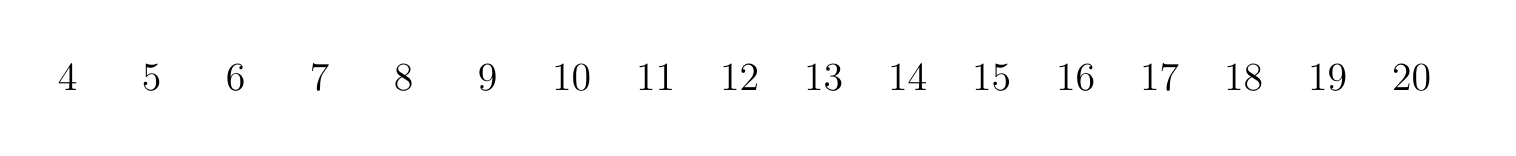
\begin{tikzpicture}[x=1in,y=1in]
\useasboundingbox (0,-0.25) rectangle (7.3,0.25);
\node[font=\Large] at (0.2,0) {4};
\node[font=\Large] at (0.62,0) {5};
\node[font=\Large] at (1.04,0) {6};
\node[font=\Large] at (1.46,0) {7};
\node[font=\Large] at (1.88,0) {8};
\node[font=\Large] at (2.3,0) {9};
\node[font=\Large] at (2.72,0) {10};
\node[font=\Large] at (3.14,0) {11};
\node[font=\Large] at (3.56,0) {12};
\node[font=\Large] at (3.98,0) {13};
\node[font=\Large] at (4.4,0) {14};
\node[font=\Large] at (4.82,0) {15};
\node[font=\Large] at (5.24,0) {16};
\node[font=\Large] at (5.66,0) {17};
\node[font=\Large] at (6.08,0) {18};
\node[font=\Large] at (6.5,0) {19};
\node[font=\Large] at (6.92,0) {20};
\end{tikzpicture}}\par
\par\vspace{0.05in}\noindent\begin{tikzpicture}[x=1in,y=1in]
\useasboundingbox (0,-2.05) rectangle (7.3,0);
\draw[black!55, line width=0.5pt] (0,-0.4) -- (7.3,-0.4);
\draw[black!55, line width=0.5pt] (0,-0.8) -- (7.3,-0.8);
\draw[black!55, line width=0.5pt] (0,-1.2) -- (7.3,-1.2);
\draw[black!55, line width=0.5pt] (0,-1.6) -- (7.3,-1.6);
\draw[black!55, line width=0.5pt] (0,-2) -- (7.3,-2);
\end{tikzpicture}\par
\vfill

\newpage
\par\vspace{0in}\noindent \prob{9} Each of these drawings was made on a ring of dots with one hop, and then the dots were erased. Find the number of dots and a hop for each drawing.\par
\par\vspace{0.35in}\noindent\makebox[\textwidth][s]{\hfill 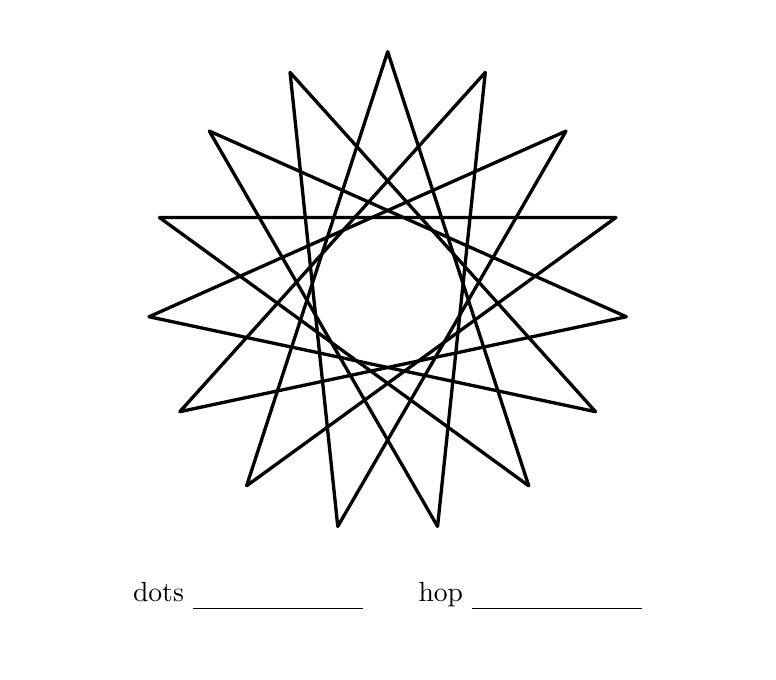
\begin{tikzpicture}[x=1in,y=1in]
\useasboundingbox (-1.8,-1.8) rectangle (1.8,1.32);
\draw[black, line width=1.2pt, line join=round] (0,1.2) -- (0.7053,-0.9708) -- (-1.1413,0.3708) -- (1.1413,0.3708) -- (-0.7053,-0.9708) -- cycle;
\draw[black, line width=1.2pt, line join=round] (0.4881,1.0963) -- (0.2495,-1.1738) -- (-0.8918,0.803) -- (1.1934,-0.1254) -- (-1.0392,-0.6) -- cycle;
\draw[black, line width=1.2pt, line join=round] (0.8918,0.803) -- (-0.2495,-1.1738) -- (-0.4881,1.0963) -- (1.0392,-0.6) -- (-1.1934,-0.1254) -- cycle;
\node[font=\normalsize] at (0,-1.52) {dots \blank\qquad hop \blank};
\end{tikzpicture}\hfill 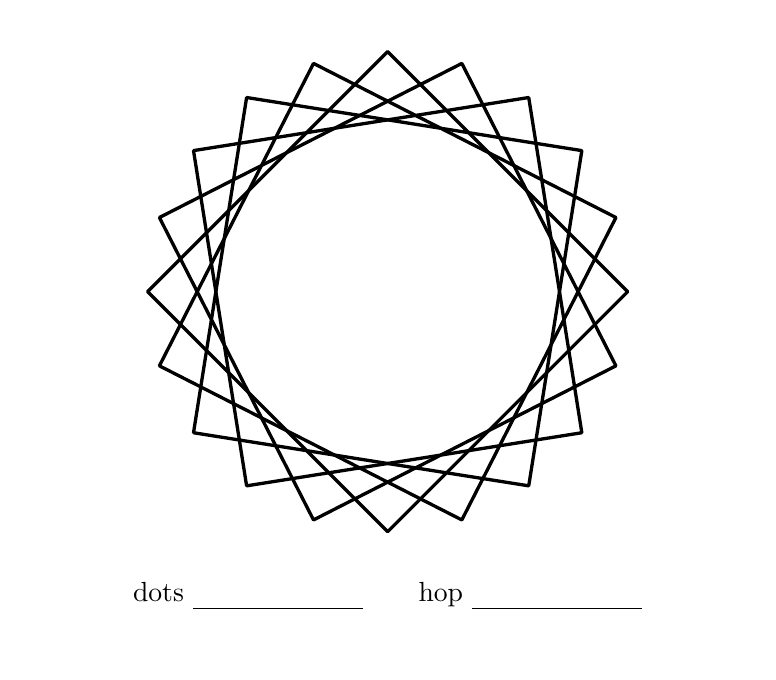
\begin{tikzpicture}[x=1in,y=1in]
\useasboundingbox (-1.8,-1.8) rectangle (1.8,1.32);
\draw[black, line width=1.2pt, line join=round] (0,1.2) -- (1.2,0) -- (0,-1.2) -- (-1.2,0) -- cycle;
\draw[black, line width=1.2pt, line join=round] (0.3708,1.1413) -- (1.1413,-0.3708) -- (-0.3708,-1.1413) -- (-1.1413,0.3708) -- cycle;
\draw[black, line width=1.2pt, line join=round] (0.7053,0.9708) -- (0.9708,-0.7053) -- (-0.7053,-0.9708) -- (-0.9708,0.7053) -- cycle;
\draw[black, line width=1.2pt, line join=round] (0.9708,0.7053) -- (0.7053,-0.9708) -- (-0.9708,-0.7053) -- (-0.7053,0.9708) -- cycle;
\draw[black, line width=1.2pt, line join=round] (1.1413,0.3708) -- (0.3708,-1.1413) -- (-1.1413,-0.3708) -- (-0.3708,1.1413) -- cycle;
\node[font=\normalsize] at (0,-1.52) {dots \blank\qquad hop \blank};
\end{tikzpicture}\hfill}\par
\par\vspace{0.5in}\noindent\makebox[\textwidth][s]{\hfill 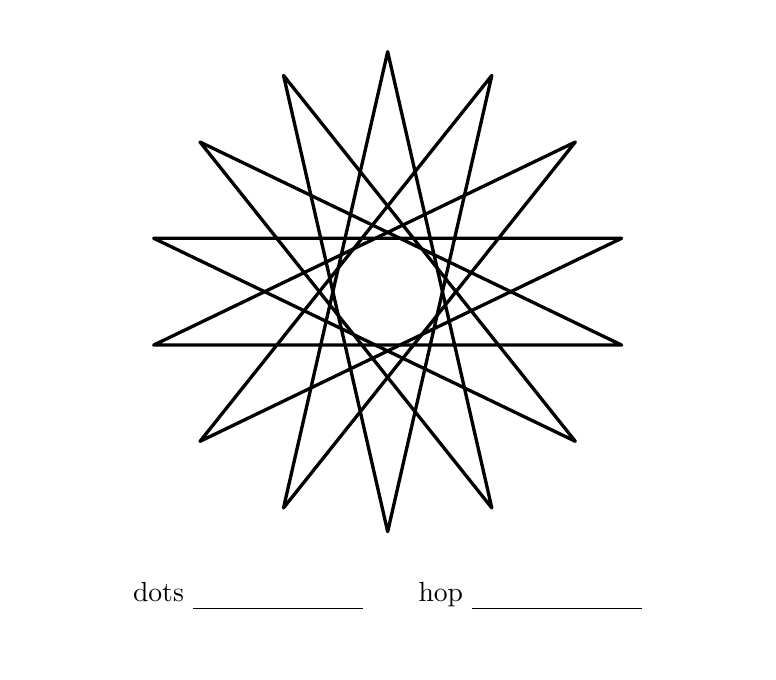
\begin{tikzpicture}[x=1in,y=1in]
\useasboundingbox (-1.8,-1.8) rectangle (1.8,1.32);
\draw[black, line width=1.2pt, line join=round] (0,1.2) -- (0.5207,-1.0812) -- (-0.9382,0.7482) -- (1.1699,-0.267) -- (-1.1699,-0.267) -- (0.9382,0.7482) -- (-0.5207,-1.0812) -- cycle;
\draw[black, line width=1.2pt, line join=round] (0.5207,1.0812) -- (0,-1.2) -- (-0.5207,1.0812) -- (0.9382,-0.7482) -- (-1.1699,0.267) -- (1.1699,0.267) -- (-0.9382,-0.7482) -- cycle;
\node[font=\normalsize] at (0,-1.52) {dots \blank\qquad hop \blank};
\end{tikzpicture}\hfill 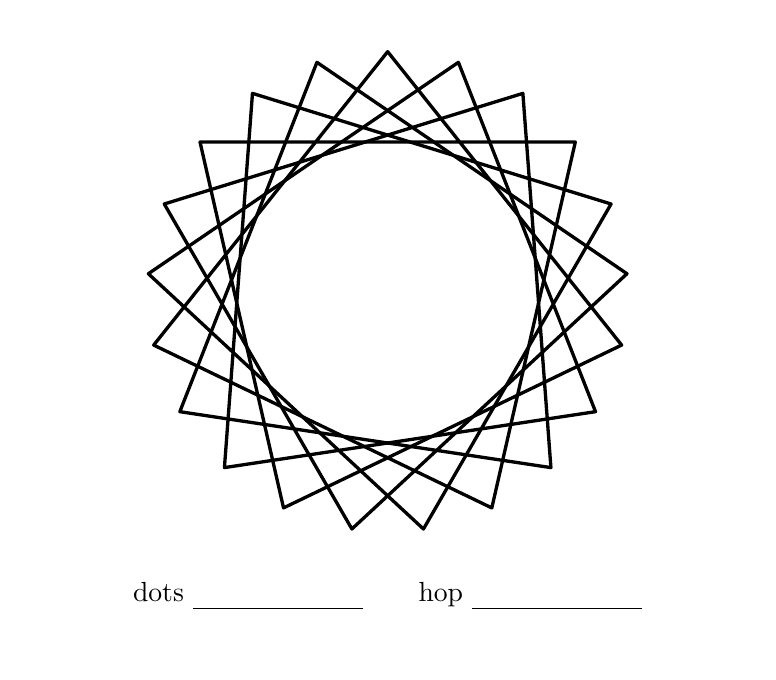
\begin{tikzpicture}[x=1in,y=1in]
\useasboundingbox (-1.8,-1.8) rectangle (1.8,1.32);
\draw[black, line width=1.2pt, line join=round] (0,1.2) -- (1.1699,-0.267) -- (-0.5207,-1.0812) -- (-0.9382,0.7482) -- (0.9382,0.7482) -- (0.5207,-1.0812) -- (-1.1699,-0.267) -- cycle;
\draw[black, line width=1.2pt, line join=round] (0.3537,1.1467) -- (1.0392,-0.6) -- (-0.8162,-0.8797) -- (-0.676,0.9915) -- (1.117,0.4384) -- (0.1789,-1.1866) -- (-1.1966,0.0897) -- cycle;
\draw[black, line width=1.2pt, line join=round] (0.676,0.9915) -- (0.8162,-0.8797) -- (-1.0392,-0.6) -- (-0.3537,1.1467) -- (1.1966,0.0897) -- (-0.1789,-1.1866) -- (-1.117,0.4384) -- cycle;
\node[font=\normalsize] at (0,-1.52) {dots \blank\qquad hop \blank};
\end{tikzpicture}\hfill}\par
\vfill

\newpage
\par\vspace{0in}\noindent \prob{10} Lee puts each message into code twice, with two different settings, so that it will be harder to crack. Explain whether this makes his messages any harder to crack.\par
\par\vspace{0.05in}\noindent\begin{tikzpicture}[x=1in,y=1in]
\useasboundingbox (0,-2.05) rectangle (7.3,0);
\draw[black!55, line width=0.5pt] (0,-0.4) -- (7.3,-0.4);
\draw[black!55, line width=0.5pt] (0,-0.8) -- (7.3,-0.8);
\draw[black!55, line width=0.5pt] (0,-1.2) -- (7.3,-1.2);
\draw[black!55, line width=0.5pt] (0,-1.6) -- (7.3,-1.6);
\draw[black!55, line width=0.5pt] (0,-2) -- (7.3,-2);
\end{tikzpicture}\par
\par\vspace{0.45in}\noindent \prob{11} Set the wheel to C. Put A into code, then put the new letter into code, and keep going until you get back to A. Which settings take A through all 26 letters before it comes back? Explain why your list is complete.\par
\par\vspace{0.05in}\noindent\begin{tikzpicture}[x=1in,y=1in]
\useasboundingbox (0,-3.65) rectangle (7.3,0);
\draw[black!55, line width=0.5pt] (0,-0.4) -- (7.3,-0.4);
\draw[black!55, line width=0.5pt] (0,-0.8) -- (7.3,-0.8);
\draw[black!55, line width=0.5pt] (0,-1.2) -- (7.3,-1.2);
\draw[black!55, line width=0.5pt] (0,-1.6) -- (7.3,-1.6);
\draw[black!55, line width=0.5pt] (0,-2) -- (7.3,-2);
\draw[black!55, line width=0.5pt] (0,-2.4) -- (7.3,-2.4);
\draw[black!55, line width=0.5pt] (0,-2.8) -- (7.3,-2.8);
\draw[black!55, line width=0.5pt] (0,-3.2) -- (7.3,-3.2);
\draw[black!55, line width=0.5pt] (0,-3.6) -- (7.3,-3.6);
\end{tikzpicture}\par
\vfill

\newpage
\par\vspace{0in}\noindent \prob{12} On the ring marked \texttimes2, draw a line from each dot to the dot with twice its number, counting on around the ring past 23 when you need to, so that dot 13 joins dot 2. On the ring marked \texttimes3, draw a line from each dot to the dot with three times its number. A dot that lands on itself gets no line.\par
\par\vspace{0.3in}\noindent\makebox[\textwidth][c]{\begin{tikzpicture}[x=1in,y=1in]
\useasboundingbox (0,-8.09) rectangle (7.3,0);
\draw[black!25, line width=0.5pt] (2.17,-2.17) circle (1.85);
\fill[black] (2.17,-0.32) circle (0.035);
\node[font=\footnotesize] at (2.17,-0.12) {0};
\fill[black] (2.6488,-0.383) circle (0.035);
\node[font=\footnotesize] at (2.7006,-0.1899) {1};
\fill[black] (3.095,-0.5679) circle (0.035);
\node[font=\footnotesize] at (3.195,-0.3946) {2};
\fill[black] (3.4781,-0.8619) circle (0.035);
\node[font=\footnotesize] at (3.6196,-0.7204) {3};
\fill[black] (3.7721,-1.245) circle (0.035);
\node[font=\footnotesize] at (3.9454,-1.145) {4};
\fill[black] (3.957,-1.6912) circle (0.035);
\node[font=\footnotesize] at (4.1501,-1.6394) {5};
\fill[black] (4.02,-2.17) circle (0.035);
\node[font=\footnotesize] at (4.22,-2.17) {6};
\fill[black] (3.957,-2.6488) circle (0.035);
\node[font=\footnotesize] at (4.1501,-2.7006) {7};
\fill[black] (3.7721,-3.095) circle (0.035);
\node[font=\footnotesize] at (3.9454,-3.195) {8};
\fill[black] (3.4781,-3.4781) circle (0.035);
\node[font=\footnotesize] at (3.6196,-3.6196) {9};
\fill[black] (3.095,-3.7721) circle (0.035);
\node[font=\footnotesize] at (3.195,-3.9454) {10};
\fill[black] (2.6488,-3.957) circle (0.035);
\node[font=\footnotesize] at (2.7006,-4.1501) {11};
\fill[black] (2.17,-4.02) circle (0.035);
\node[font=\footnotesize] at (2.17,-4.22) {12};
\fill[black] (1.6912,-3.957) circle (0.035);
\node[font=\footnotesize] at (1.6394,-4.1501) {13};
\fill[black] (1.245,-3.7721) circle (0.035);
\node[font=\footnotesize] at (1.145,-3.9454) {14};
\fill[black] (0.8619,-3.4781) circle (0.035);
\node[font=\footnotesize] at (0.7204,-3.6196) {15};
\fill[black] (0.5679,-3.095) circle (0.035);
\node[font=\footnotesize] at (0.3946,-3.195) {16};
\fill[black] (0.383,-2.6488) circle (0.035);
\node[font=\footnotesize] at (0.1899,-2.7006) {17};
\fill[black] (0.32,-2.17) circle (0.035);
\node[font=\footnotesize] at (0.12,-2.17) {18};
\fill[black] (0.383,-1.6912) circle (0.035);
\node[font=\footnotesize] at (0.1899,-1.6394) {19};
\fill[black] (0.5679,-1.245) circle (0.035);
\node[font=\footnotesize] at (0.3946,-1.145) {20};
\fill[black] (0.8619,-0.8619) circle (0.035);
\node[font=\footnotesize] at (0.7204,-0.7204) {21};
\fill[black] (1.245,-0.5679) circle (0.035);
\node[font=\footnotesize] at (1.145,-0.3946) {22};
\fill[black] (1.6912,-0.383) circle (0.035);
\node[font=\footnotesize] at (1.6394,-0.1899) {23};
\node[font=\LARGE] at (4.65,-0.35) {\texttimes2};
\draw[black!25, line width=0.5pt] (5.13,-5.92) circle (1.85);
\fill[black] (5.13,-4.07) circle (0.035);
\node[font=\footnotesize] at (5.13,-3.87) {0};
\fill[black] (5.6088,-4.133) circle (0.035);
\node[font=\footnotesize] at (5.6606,-3.9399) {1};
\fill[black] (6.055,-4.3179) circle (0.035);
\node[font=\footnotesize] at (6.155,-4.1446) {2};
\fill[black] (6.4381,-4.6119) circle (0.035);
\node[font=\footnotesize] at (6.5796,-4.4704) {3};
\fill[black] (6.7321,-4.995) circle (0.035);
\node[font=\footnotesize] at (6.9054,-4.895) {4};
\fill[black] (6.917,-5.4412) circle (0.035);
\node[font=\footnotesize] at (7.1101,-5.3894) {5};
\fill[black] (6.98,-5.92) circle (0.035);
\node[font=\footnotesize] at (7.18,-5.92) {6};
\fill[black] (6.917,-6.3988) circle (0.035);
\node[font=\footnotesize] at (7.1101,-6.4506) {7};
\fill[black] (6.7321,-6.845) circle (0.035);
\node[font=\footnotesize] at (6.9054,-6.945) {8};
\fill[black] (6.4381,-7.2281) circle (0.035);
\node[font=\footnotesize] at (6.5796,-7.3696) {9};
\fill[black] (6.055,-7.5221) circle (0.035);
\node[font=\footnotesize] at (6.155,-7.6954) {10};
\fill[black] (5.6088,-7.707) circle (0.035);
\node[font=\footnotesize] at (5.6606,-7.9001) {11};
\fill[black] (5.13,-7.77) circle (0.035);
\node[font=\footnotesize] at (5.13,-7.97) {12};
\fill[black] (4.6512,-7.707) circle (0.035);
\node[font=\footnotesize] at (4.5994,-7.9001) {13};
\fill[black] (4.205,-7.5221) circle (0.035);
\node[font=\footnotesize] at (4.105,-7.6954) {14};
\fill[black] (3.8219,-7.2281) circle (0.035);
\node[font=\footnotesize] at (3.6804,-7.3696) {15};
\fill[black] (3.5279,-6.845) circle (0.035);
\node[font=\footnotesize] at (3.3546,-6.945) {16};
\fill[black] (3.343,-6.3988) circle (0.035);
\node[font=\footnotesize] at (3.1499,-6.4506) {17};
\fill[black] (3.28,-5.92) circle (0.035);
\node[font=\footnotesize] at (3.08,-5.92) {18};
\fill[black] (3.343,-5.4412) circle (0.035);
\node[font=\footnotesize] at (3.1499,-5.3894) {19};
\fill[black] (3.5279,-4.995) circle (0.035);
\node[font=\footnotesize] at (3.3546,-4.895) {20};
\fill[black] (3.8219,-4.6119) circle (0.035);
\node[font=\footnotesize] at (3.6804,-4.4704) {21};
\fill[black] (4.205,-4.3179) circle (0.035);
\node[font=\footnotesize] at (4.105,-4.1446) {22};
\fill[black] (4.6512,-4.133) circle (0.035);
\node[font=\footnotesize] at (4.5994,-3.9399) {23};
\node[font=\LARGE] at (2.63,-7.77) {\texttimes3};
\end{tikzpicture}}\par
\vfill

\newpage
\par\vspace{0in}\noindent\makebox[\textwidth][c]{\begin{tikzpicture}[x=1in,y=1in]
\useasboundingbox (0,0) rectangle (7.3,8.9);
\draw[line width=1.4pt] (3.65,4.45) circle (2.75);
\node[font=\bfseries\LARGE, rotate=0] at (3.65,6.88) {\underline{A}};
\draw[line width=0.6pt] (3.9007,6.5148) -- (3.9815,7.1799);
\node[font=\bfseries\LARGE, rotate=-13.8462] at (4.2315,6.8094) {\underline{B}};
\draw[line width=0.6pt] (4.3876,6.3948) -- (4.6252,7.0213);
\node[font=\bfseries\LARGE, rotate=-27.6923] at (4.7793,6.6017) {\underline{C}};
\draw[line width=0.6pt] (4.8316,6.1618) -- (5.2122,6.7132);
\node[font=\bfseries\LARGE, rotate=-41.5385] at (5.2614,6.2689) {\underline{D}};
\draw[line width=0.6pt] (5.2069,5.8293) -- (5.7084,6.2736);
\node[font=\bfseries\LARGE, rotate=-55.3846] at (5.6499,5.8304) {\underline{E}};
\draw[line width=0.6pt] (5.4917,5.4166) -- (6.085,5.728);
\node[font=\bfseries\LARGE, rotate=-69.2308] at (5.9221,5.3117) {\underline{F}};
\draw[line width=0.6pt] (5.6696,4.9478) -- (6.3201,5.1081);
\node[font=\bfseries\LARGE, rotate=-83.0769] at (6.0623,4.7429) {\underline{G}};
\draw[line width=0.6pt] (5.73,4.45) -- (6.4,4.45);
\node[font=\bfseries\LARGE, rotate=-96.9231] at (6.0623,4.1571) {\underline{H}};
\draw[line width=0.6pt] (5.6696,3.9522) -- (6.3201,3.7919);
\node[font=\bfseries\LARGE, rotate=-110.7692] at (5.9221,3.5883) {\underline{I}};
\draw[line width=0.6pt] (5.4917,3.4834) -- (6.085,3.172);
\node[font=\bfseries\LARGE, rotate=-124.6154] at (5.6499,3.0696) {\underline{J}};
\draw[line width=0.6pt] (5.2069,3.0707) -- (5.7084,2.6264);
\node[font=\bfseries\LARGE, rotate=-138.4615] at (5.2614,2.6311) {\underline{K}};
\draw[line width=0.6pt] (4.8316,2.7382) -- (5.2122,2.1868);
\node[font=\bfseries\LARGE, rotate=-152.3077] at (4.7793,2.2983) {\underline{L}};
\draw[line width=0.6pt] (4.3876,2.5052) -- (4.6252,1.8787);
\node[font=\bfseries\LARGE, rotate=-166.1538] at (4.2315,2.0906) {\underline{M}};
\draw[line width=0.6pt] (3.9007,2.3852) -- (3.9815,1.7201);
\node[font=\bfseries\LARGE, rotate=-180] at (3.65,2.02) {\underline{N}};
\draw[line width=0.6pt] (3.3993,2.3852) -- (3.3185,1.7201);
\node[font=\bfseries\LARGE, rotate=-193.8462] at (3.0685,2.0906) {\underline{O}};
\draw[line width=0.6pt] (2.9124,2.5052) -- (2.6748,1.8787);
\node[font=\bfseries\LARGE, rotate=-207.6923] at (2.5207,2.2983) {\underline{P}};
\draw[line width=0.6pt] (2.4684,2.7382) -- (2.0878,2.1868);
\node[font=\bfseries\LARGE, rotate=-221.5385] at (2.0386,2.6311) {\underline{Q}};
\draw[line width=0.6pt] (2.0931,3.0707) -- (1.5916,2.6264);
\node[font=\bfseries\LARGE, rotate=-235.3846] at (1.6501,3.0696) {\underline{R}};
\draw[line width=0.6pt] (1.8083,3.4834) -- (1.215,3.172);
\node[font=\bfseries\LARGE, rotate=-249.2308] at (1.3779,3.5883) {\underline{S}};
\draw[line width=0.6pt] (1.6304,3.9522) -- (0.9799,3.7919);
\node[font=\bfseries\LARGE, rotate=-263.0769] at (1.2377,4.1571) {\underline{T}};
\draw[line width=0.6pt] (1.57,4.45) -- (0.9,4.45);
\node[font=\bfseries\LARGE, rotate=-276.9231] at (1.2377,4.7429) {\underline{U}};
\draw[line width=0.6pt] (1.6304,4.9478) -- (0.9799,5.1081);
\node[font=\bfseries\LARGE, rotate=-290.7692] at (1.3779,5.3117) {\underline{V}};
\draw[line width=0.6pt] (1.8083,5.4166) -- (1.215,5.728);
\node[font=\bfseries\LARGE, rotate=-304.6154] at (1.6501,5.8304) {\underline{W}};
\draw[line width=0.6pt] (2.0931,5.8293) -- (1.5916,6.2736);
\node[font=\bfseries\LARGE, rotate=-318.4615] at (2.0386,6.2689) {\underline{X}};
\draw[line width=0.6pt] (2.4684,6.1618) -- (2.0878,6.7132);
\node[font=\bfseries\LARGE, rotate=-332.3077] at (2.5207,6.6017) {\underline{Y}};
\draw[line width=0.6pt] (2.9124,6.3948) -- (2.6748,7.0213);
\node[font=\bfseries\LARGE, rotate=-346.1538] at (3.0685,6.8094) {\underline{Z}};
\draw[line width=0.6pt] (3.3993,6.5148) -- (3.3185,7.1799);
\fill (3.65,4.45) circle (0.05);
\draw[line width=0.6pt] (3.47,4.45) -- (3.83,4.45) (3.65,4.27) -- (3.65,4.63);
\end{tikzpicture}}\par
\vfill

\newpage
\par\vspace{0in}\noindent\makebox[\textwidth][c]{\begin{tikzpicture}[x=1in,y=1in]
\useasboundingbox (0,0) rectangle (7.3,8.9);
\draw[line width=1.4pt] (3.65,4.45) circle (2);
\node[font=\bfseries\Large, rotate=0] at (3.65,6.15) {\underline{A}};
\draw[line width=0.6pt] (3.8212,5.8596) -- (3.8911,6.4354);
\node[font=\bfseries\Large, rotate=-13.8462] at (4.0568,6.1006) {\underline{B}};
\draw[line width=0.6pt] (4.1535,5.7777) -- (4.3592,6.32);
\node[font=\bfseries\Large, rotate=-27.6923] at (4.44,5.9553) {\underline{C}};
\draw[line width=0.6pt] (4.4567,5.6186) -- (4.7861,6.096);
\node[font=\bfseries\Large, rotate=-41.5385] at (4.7773,5.7225) {\underline{D}};
\draw[line width=0.6pt] (4.7129,5.3916) -- (5.147,5.7762);
\node[font=\bfseries\Large, rotate=-55.3846] at (5.0491,5.4157) {\underline{E}};
\draw[line width=0.6pt] (4.9073,5.1099) -- (5.4209,5.3794);
\node[font=\bfseries\Large, rotate=-69.2308] at (5.2395,5.0528) {\underline{F}};
\draw[line width=0.6pt] (5.0287,4.7898) -- (5.5919,4.9286);
\node[font=\bfseries\Large, rotate=-83.0769] at (5.3376,4.6549) {\underline{G}};
\draw[line width=0.6pt] (5.07,4.45) -- (5.65,4.45);
\node[font=\bfseries\Large, rotate=-96.9231] at (5.3376,4.2451) {\underline{H}};
\draw[line width=0.6pt] (5.0287,4.1102) -- (5.5919,3.9714);
\node[font=\bfseries\Large, rotate=-110.7692] at (5.2395,3.8472) {\underline{I}};
\draw[line width=0.6pt] (4.9073,3.7901) -- (5.4209,3.5206);
\node[font=\bfseries\Large, rotate=-124.6154] at (5.0491,3.4843) {\underline{J}};
\draw[line width=0.6pt] (4.7129,3.5084) -- (5.147,3.1238);
\node[font=\bfseries\Large, rotate=-138.4615] at (4.7773,3.1775) {\underline{K}};
\draw[line width=0.6pt] (4.4567,3.2814) -- (4.7861,2.804);
\node[font=\bfseries\Large, rotate=-152.3077] at (4.44,2.9447) {\underline{L}};
\draw[line width=0.6pt] (4.1535,3.1223) -- (4.3592,2.58);
\node[font=\bfseries\Large, rotate=-166.1538] at (4.0568,2.7994) {\underline{M}};
\draw[line width=0.6pt] (3.8212,3.0404) -- (3.8911,2.4646);
\node[font=\bfseries\Large, rotate=-180] at (3.65,2.75) {\underline{N}};
\draw[line width=0.6pt] (3.4788,3.0404) -- (3.4089,2.4646);
\node[font=\bfseries\Large, rotate=-193.8462] at (3.2432,2.7994) {\underline{O}};
\draw[line width=0.6pt] (3.1465,3.1223) -- (2.9408,2.58);
\node[font=\bfseries\Large, rotate=-207.6923] at (2.86,2.9447) {\underline{P}};
\draw[line width=0.6pt] (2.8433,3.2814) -- (2.5139,2.804);
\node[font=\bfseries\Large, rotate=-221.5385] at (2.5227,3.1775) {\underline{Q}};
\draw[line width=0.6pt] (2.5871,3.5084) -- (2.153,3.1238);
\node[font=\bfseries\Large, rotate=-235.3846] at (2.2509,3.4843) {\underline{R}};
\draw[line width=0.6pt] (2.3927,3.7901) -- (1.8791,3.5206);
\node[font=\bfseries\Large, rotate=-249.2308] at (2.0605,3.8472) {\underline{S}};
\draw[line width=0.6pt] (2.2713,4.1102) -- (1.7081,3.9714);
\node[font=\bfseries\Large, rotate=-263.0769] at (1.9624,4.2451) {\underline{T}};
\draw[line width=0.6pt] (2.23,4.45) -- (1.65,4.45);
\node[font=\bfseries\Large, rotate=-276.9231] at (1.9624,4.6549) {\underline{U}};
\draw[line width=0.6pt] (2.2713,4.7898) -- (1.7081,4.9286);
\node[font=\bfseries\Large, rotate=-290.7692] at (2.0605,5.0528) {\underline{V}};
\draw[line width=0.6pt] (2.3927,5.1099) -- (1.8791,5.3794);
\node[font=\bfseries\Large, rotate=-304.6154] at (2.2509,5.4157) {\underline{W}};
\draw[line width=0.6pt] (2.5871,5.3916) -- (2.153,5.7762);
\node[font=\bfseries\Large, rotate=-318.4615] at (2.5227,5.7225) {\underline{X}};
\draw[line width=0.6pt] (2.8433,5.6186) -- (2.5139,6.096);
\node[font=\bfseries\Large, rotate=-332.3077] at (2.86,5.9553) {\underline{Y}};
\draw[line width=0.6pt] (3.1465,5.7777) -- (2.9408,6.32);
\node[font=\bfseries\Large, rotate=-346.1538] at (3.2432,6.1006) {\underline{Z}};
\draw[line width=0.6pt] (3.4788,5.8596) -- (3.4089,6.4354);
\fill (3.65,4.45) circle (0.05);
\draw[line width=0.6pt] (3.47,4.45) -- (3.83,4.45) (3.65,4.27) -- (3.65,4.63);
\end{tikzpicture}}\par
\vfill

\end{document}
